\documentclass[11pt]{article}
\usepackage{geometry}                
\geometry{letterpaper}                 
\usepackage[parfill]{parskip}        
\usepackage{graphicx}
\usepackage{amssymb}
\usepackage{amsmath}
\usepackage{epstopdf}
\usepackage{verbatim}
\usepackage{float}
\usepackage{enumerate}
\usepackage{hyperref}
\usepackage[utf8]{inputenc}
\usepackage[T1]{fontenc}
\DeclareGraphicsRule{.tif}{png}{.png}{`convert #1 `dirname #1`/`basename #1 .tif`.png}
\usepackage{color}
\usepackage{textcomp}
\definecolor{listinggray}{gray}{0.9}
\definecolor{lbcolor}{rgb}{1,1,1}

\begin{document}
{\small
\section*{Problems for Discussion 5, 10/23/13}
Compiled by Mai Le, some problems from Prof. Fessler, Daehyun Yoon
}

\section{Alternative Sampling Theorem}
% Fessler 556, hmwk 3, p4

Generalize the ideal impulse sampling theory to the more realistic case to account for finite detector size:

\[
g_d[n] = \frac{1}{T}\int_{(n-\frac{1}{2})T}^{(n+\frac{1}{2})T} g_c(t) dt
\]

{\color{blue}
The main results of Shannon/Nyquist's sampling theorem (for ideal sampling) addresses the following three questions:
\begin{itemize}
	\item Q1: Can we recover a bandlimited signal from its samples? \\
	\quad A1: Yes, if it is bandlimited and sampled correctly.
	\item Q2: How "fast" must we sample? \\
	\quad A2: The required sampling frequency is twice the highest signal frequency.
	\item Q3: How do we recover the analog signal from its samples? \\
	\quad A3: In the frequency domain, $G_a(\Omega) = G_s(\Omega) rect(\Omega T)$, or equivalently since interpolation in the time domain.
\end{itemize}

For this more realistic sampling method, we are integrating over the time between samples. This is equivalent to filtering the signal with a rect function before sampling. Let's call that filtered signal $f(t)$. 

\begin{eqnarray*}
\text{Let } r(t) &=& \frac{1}{T} rect\left(\frac{t}{T}\right) \\
f(t) = r(t) * g_c(t) &=& \int_{-\infty}^\infty g_c(\tau) r(t-\tau) d\tau \\
&=& \int_{-\infty}^\infty g_c(\tau) \frac{1}{T} rect\left(\frac{t-\tau}{T}\right) d\tau \\
&=& \frac{1}{T}  \int_{t-\frac{T}{2}}^{t+\frac{T}{2}} g_c(\tau) d\tau \\
\end{eqnarray*}

Now consider samples of $f(t)$, called $f_d[n]$. Also let $f_s(n) = comb\left(\frac{t}{T}\right) \cdot f(t)$.

\begin{eqnarray*}
f_d[n] &=& f(nT) = f_s(nT) \\
&=& \frac{1}{T}  \int_{nT-\frac{T}{2}}^{nT+\frac{T}{2}} g_c(\tau) d\tau \\
&=& \frac{1}{T}  \int_{\left(n-\frac{1}{2}\right)T}^{\left(n+\frac{1}{2}\right)T} g_c(t) dt  = g_d[n]\\
\end{eqnarray*}

Thus I have shown that the samples $g_d[n]$ acquired with this more realistic sensor are equivalent to the ideal samples $f_d[n]$ of the filtered signal $f(t) = r(t)*g_c(t)$. This means we can use the results from the Shannon-Nyquist sampling theorem for ideal sampling!

But first, we need to see how this filter changes the CTFT of $g_c(t)$, $G_c(\Omega)$. Assuming $G_c(\Omega)$ is bandlimited with maximum frequency $\Omega_c$, then is $F(\Omega)$ also bandlimited? If so, what is its maximum frequency?

From the convolution theorem, 
\[
F(\Omega) = G_c(\Omega)R(\Omega)
\]

and from known Fourier Transform pairs, 

\[
R(\Omega) = sinc(T \Omega).
\]

Assuming $T$ is small, this is a pretty wide sinc, with its first set of zeros far out, at $\pm \frac{1}{T}$. So the maximum frequency for $F(\Omega)$ is $min(\frac{1}{T}, \Omega_c)$. In most cases, $T$ will be large enough that the maximum frequency for $F\Omega)$ is $\Omega_c$, same as for $G_c(\Omega)$.

So now we re-address the three questions answered in the sampling theorem:
\begin{itemize}
	\item Q1: Can we recover a bandlimited signal ($g_c[n]$) from its samples? \\
	\quad A1: Yes, if $g_c[n]$ is bandlimited and sampled correctly.
	\item Q2: How "fast" must we sample? \\
	\quad A2: The required sampling frequency is twice the highest signal frequency of $F(\Omega)$, $min(\frac{1}{T}, \Omega_c)$.
	\item Q3: How do we recover the analog signal from its samples? \\
	\quad A3: In the frequency domain, $F(\Omega) = F_s(\Omega) rect(\Omega T) = G_c(\Omega)R(\Omega)$ or $G_c(\Omega) = \frac{F_s(\Omega) rect(\Omega T)}{R(\Omega)}$. In other words, we need to do low-pass filtering by $\frac{1}{R(\Omega)}$ to undo the distortion from $R(\Omega)$. 
\end{itemize}
}

\section{Nyquist Rate for Communications Channel}
% Yagle Rec 2

A seismic signal with amplitude range [-1,1] volts is sampled and quantized with a 12 bit A/D converter before transmitting it over a communication channel which can support a maximum bit rate of 240 Kbits/sec. What is the maximum sampling frequency the system can support? What is the maximum frequency that can be present in the original seismic signal in order to avoid any loss of information?

{\color{blue}
We can sample at $240000/12 = 20000 Hz$. In order to avoid aliasing, the Nyquist rate of the signal should be no longer than 20000 Hz. So the maximum possible frequency is 10000 Hz.



}

\section{Sinc interpolation}
% Yagle Rec 2
A signal x(t) has a triangular spectrum, with maximum frequencies $\pm \Omega_c$ and height $A$. x(t) is sampled at a rate of $f_s = \frac{1}{T_s}=\frac{\Omega_s}{2 \pi}$, producing the samples $\{x(nT_s)\}_{n=-\infty}^\infty$.

Let $y(t)$ be the signal constructed from these samples as follows:
\[
y(t) = \frac{ \Omega_c T_s}{\pi} \sum_{n=-\infty}^\infty x(nT_s) sinc\left( \frac{\Omega_c}{\pi} (t-nT_s) \right)
\]

How is $y(t)$ related to $x(t)$ when:

(a) $\Omega_c = \frac{\Omega_s}{4}$ 

{\color{blue}
\begin{eqnarray*}
y(t) &=& \frac{ \omega_c T_s}{\pi} \sum_{n=-\infty}^\infty x(nT_s) sinc\left( \frac{\Omega_c}{\pi} (t-nT_s) \right) \\
&=& \left(\sum_n x(nT_s) \delta(t-nT_s) \right)*\left(sinc\left(\frac{\Omega_c t}{\pi}\right)\frac{\Omega_c T_s}{\pi} \right) \\
Y(\Omega) &=& \frac{1}{T_s} \left( \sum_{n=-\infty}^\infty X(\Omega - \Omega_s n) \right) H(\Omega)\\
\end{eqnarray*}

where $H(\Omega) = T_s rect(\frac{ \Omega}{2 \Omega_C})$.

%\[
%\frac{\Omega_c T_s}{\pi} sinc\left(\frac{\Omega_c t}{\pi}\right) \leftrightarrow \frac{\Omega_c T_s}{\pi} \left[\frac{\pi}{\Omega_c} rect\left(\frac{\pi \Omega}{2 \pi \Omega_C}\right) \right] = T_s rect\left(\frac{\Omega}{2 \Omega_C}\right) 
%\]

Thus, we can interpret the CTFT of $y(t)$ as a low-pass filter applied to a series of replicas of $X(\Omega)$.

So for $\Omega_c = \frac{\Omega_s}{4}$, the replicas have width $2\Omega_c$ and are placed $4\Omega_c$ apart, with space of $2\Omega_c$ in between. There is no aliasing, so we are able to perfectly recover the central replica, $Y(\Omega) = X(\Omega)$, and thus recover the original signal $y[n]=x[n]$. 

}

(b) $\Omega_c = \Omega_s$?

{\color{blue}
This sampling rate does not satisfy the Nyquist rate. The replicas are spaced only $\Omega_c$ apart, each pair of replicas having an overlap region of width $\Omega_c$. In fact, the entire domain $\Omega$ suffers from aliasing, and our attempt to recover the original signal results in $Y(\Omega) = Arect\left(\frac{\Omega}{2\Omega_c} \right) \neq X(\Omega)$.
}

\section{Relating CTFT and DTFT}
% Pradhan disc

Suppose the CTFT of the continuous time signal $x_a(t)$ is as following.

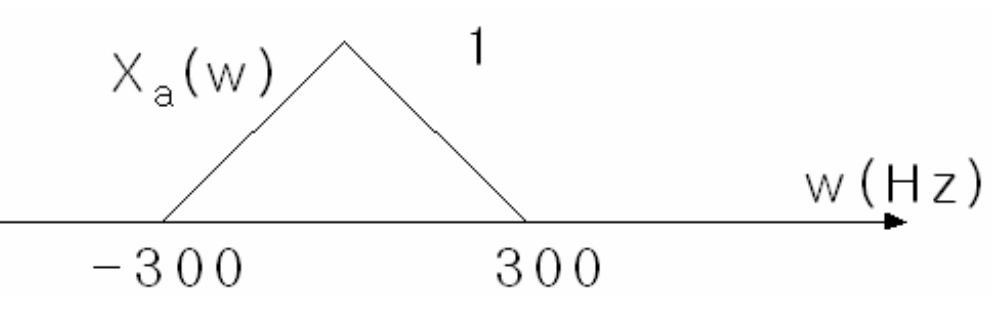
\includegraphics[width = 0.8\textwidth]{CTFT_p4.png} 

Determine the DTFT of the sampled signal $x[n]$, when the sampling period is 1 ms. What happens if the sampling period is 2 ms?


{\color{blue}
First we compute the baseband by multiplying $2 \pi T_s = 2 \pi 0.001 = \frac{\pi}{500}$. Next we scale the amplitude by $\frac{1}{T_s} = 1000$. 

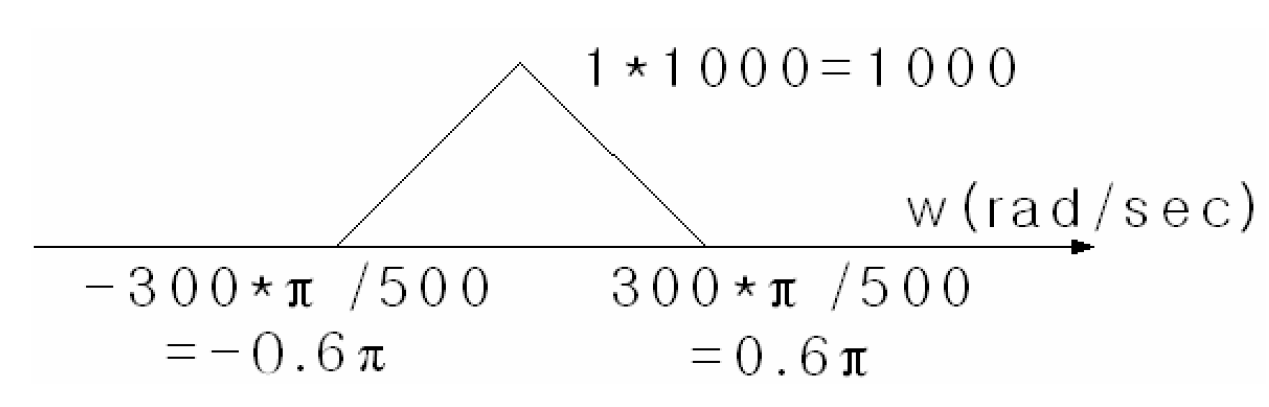
\includegraphics[width = 0.8\textwidth]{CTFT_p4_a.png} 

Next we create copies of the above baseband signal by shifting it to every multiple of $2 \pi$. For example, shift it by $2 \pi$ for one copy and shift it by $4 \pi$ to get another copy and so on. Summing these copies together we get $X_d(\omega)$:

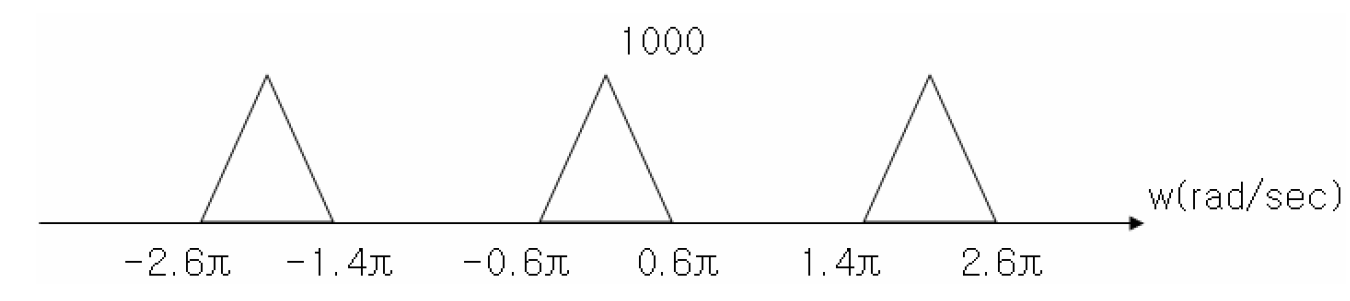
\includegraphics[width = 0.8\textwidth]{CTFT_p4_d.png} 

}

\end{document}